% This file was created by matlab2tikz.
%
%The latest updates can be retrieved from
%  http://www.mathworks.com/matlabcentral/fileexchange/22022-matlab2tikz-matlab2tikz
%where you can also make suggestions and rate matlab2tikz.
%
\documentclass[tikz]{standalone}
\usepackage[T1]{fontenc}
\usepackage[utf8]{inputenc}
\usepackage{pgfplots}
\usepackage{grffile}
\pgfplotsset{compat=newest}
\usetikzlibrary{plotmarks}
\usepgfplotslibrary{patchplots}
\usepackage{amsmath}
\usetikzlibrary{decorations.markings}
\usetikzlibrary{math}

\begin{document}
		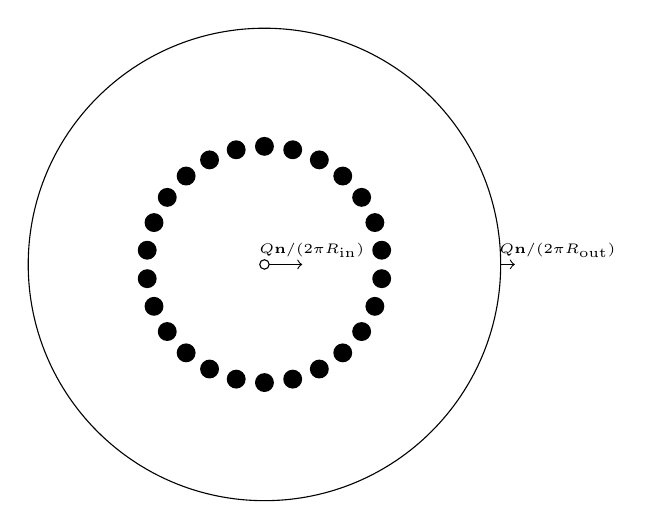
\begin{tikzpicture}[scale=0.6]
		\draw(0,0)circle(0.1);
		\draw(0,0)circle(5);
		\foreach \n in {0,...,25}
			{
				\fill({2.5*sin(360/26*\n)},{2.5*cos(360/26*\n)}) circle(0.2);
			} 
		 \draw[->](0.1,0)--(0.8,0);
		\draw(1,0.3) node {\tiny$Q \mathbf{n}/(2\pi R_{\text{in}})$};
		 \draw[->](5,0)--(5.3,0);
		\draw(6.2,0.3) node {\tiny$Q \mathbf{n}/(2\pi R_{\text{out}})$};
\end{tikzpicture}
\end{document}